\section{Żadanie adresacji}
Tutaj po raz pierwszy można zaobserwować zmienioną wartość pola adresu dla wiadomości
przychodzącej. Oznacza to, że urządzenie podrzędne zaakceptowało żadanie adresacji 
oraz identyfikuje się w trakcie rozmowy z urządzeniem nadrzędnym pod adresem 0x03 co
jest prawdą dla każdej następnej wiadomości.

identyfikujące się unikalnym identyfikatorem \textit{UniqueID} == \{0x4E, 0x4B, 0x34, 0x36, 0x35, 0x30, 0x30, 0x30, 0x30\}
\begin{figure}[h!]
    \centering
    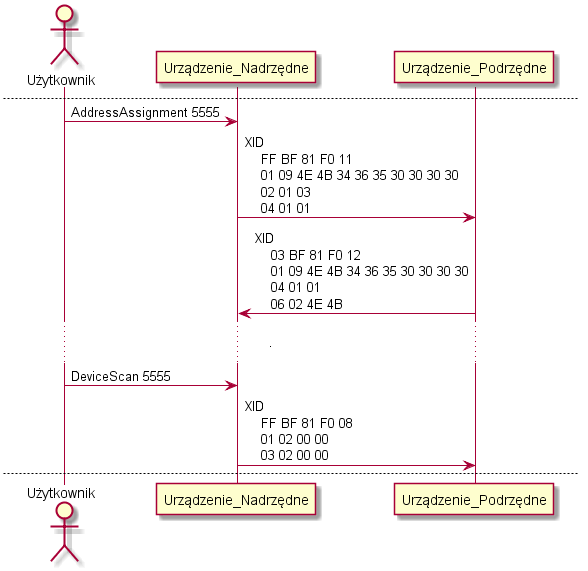
\includegraphics[scale=0.75]{out/Diagramy/UML_DiagramOfSequence_New/UML_DiagramOfSequence_New-page2.png}
    \caption{Żadanie adresacji oraz dodatkowe skanowanie urządzeń.
        \newline(Opracowanie własne)}
    \label{fig:DiagramSequence_AddressAssignment_SecondDeviceScan}
\end{figure}
